%%%%%%%%%%%%%%%%%%%%%%% file template.tex %%%%%%%%%%%%%%%%%%%%%%%%%
%
% This is a general template file for the LaTeX package SVJour3
% for Springer journals.          Springer Heidelberg 2010/09/16
%
% Copy it to a new file with a new name and use it as the basis
% for your article. Delete % signs as needed.
%
% This template includes a few options for different layouts and
% content for various journals. Please consult a previous issue of
% your journal as needed.
%
%%%%%%%%%%%%%%%%%%%%%%%%%%%%%%%%%%%%%%%%%%%%%%%%%%%%%%%%%%%%%%%%%%%
%
% First comes an example EPS file -- just ignore it and
% proceed on the \documentclass line
% your LaTeX will extract the file if required
\begin{filecontents*}{example.eps}
%!PS-Adobe-3.0 EPSF-3.0
%%BoundingBox: 19 19 221 221
%%CreationDate: Mon Sep 29 1997
%%Creator: programmed by hand (JK)
%%EndComments
gsave
newpath
  20 20 moveto
  20 220 lineto
  220 220 lineto
  220 20 lineto
closepath
2 setlinewidth
gsave
  .4 setgray fill
grestore
stroke
grestore
\end{filecontents*}
%
\RequirePackage{fix-cm}
%
%\documentclass{svjour3}                     % onecolumn (standard format)
%\documentclass[smallcondensed]{svjour3}     % onecolumn (ditto)
%\documentclass[smallextended]{svjour3}       % onecolumn (second format)
\documentclass[twocolumn]{svjour3}          % twocolumn
%
\smartqed  % flush right qed marks, e.g. at end of proof
%
\usepackage{graphicx}
\usepackage{array}
\usepackage{color}
\usepackage{flexisym}
%
% \usepackage{mathptmx}      % use Times fonts if available on your TeX system
%
% insert here the call for the packages your document requires
%\usepackage{latexsym}
% etc.
%
% please place your own definitions here and don't use \def but
% \newcommand{}{}
%
% Insert the name of "your journal" with
% \journalname{myjournal}
%
\begin{document}

\begin{sloppy}

\title{Intelligent Virtual Agents and Spoken Dialog Systems come together to Deliver Brief Health Interventions\thanks{Part of this research was funded by grants from the National Science Foundation HRD-0833093, IIP-1338922, IIP- 1237818.}
}
%\subtitle{Do you have a subtitle?\\ If so, write it here}

\titlerunning{Spoken Dialog Systems to Deliver Brief Health Interventions}        % if too long for running head

\author{        \and
         %etc.
}

%\authorrunning{Short form of author list} % if too long for running head

\institute{U. Yasavur, C. Lisetti and N. Rishe\at
              School of Computing \& Info. Sciences, Florida International University, Miami FL, 33199 \\
              Tel.: +1-305-348-6242\\
              E-mail:\{uyasa001$|$lisetti$|$rishen\}@cis.fiu.edu    
}

\date{Received: date / Accepted: date}
% The correct dates will be entered by the editor


\maketitle

\begin{abstract}
We developed a virtual counseling system which can deliver brief alcohol health interventions via a 3D anthropomorphic speech-enabled interface - a new field for spoken dialog interactions with intelligent virtual agents in the health domain. We present our spoken dialog system design and its evaluation. We developed our dialog system based on Markov decision processes (MDP) framework and optimized it by using reinforcement learning (RL) algorithms with data we collected from real user interactions. The system begins to learn optimal dialog strategies for initiative selection and for the type of confirmations that it uses during the interaction. We compared the unoptimized system with the optimized system in terms of objective measures (e.g. task completion) and subjective measures (e.g.~ease of use, future intention to use the system) and obtained positive results.

\keywords{Spoken dialog systems \and reinforcement learning \and intelligent virtual agents and avatars \and conversational agents \and alcohol \and healthy lifestyle screening \and behavior change brief intervention}
% \PACS{PACS code1 \and PACS code2 \and more}
% \subclass{MSC code1 \and MSC code2 \and more}
\end{abstract}

\section{Introduction}
\label{intro}

Intelligent virtual agents (IVA) - also known as embodied conversational agents (ECA) or virtual humans (VH) - and spoken dialog systems (SDS) are two emerging fields of research which, {\em together}, could bring a revolution to human-computer interaction as we know it. Even though the term ECA includes the notion of spoken dialog, SDS and ECA communities  still do not have a strong connection. While  progress in the spoken dialog system area is complementary for the development of conversational embodied agents,  latest findings in SDS research have not been commonly used by ECA researchers (and vice versa).

Indeed, although spoken dialog systems (SDS, henceforth) research has shown in the past few years that using Reinforcement Learning (RL) with MDPs for dialog management outperforms older hand-crafted rule-based approaches \cite{frampton2009,young2013pomdp}, intelligent virtual agent researchers have not yet integrated these results in their dialog systems.  ECA-based systems usually involve spoken dialog (versus menu options to choose from), but their dialog management usually still relies on hand-crafted methods \cite{morbiniFlores2012,Bickmore2010}.

% For two-column wide figures use
%\begin{figure*}
% Use the relevant command to insert your figure file.
% For example, with the graphicx package use
%  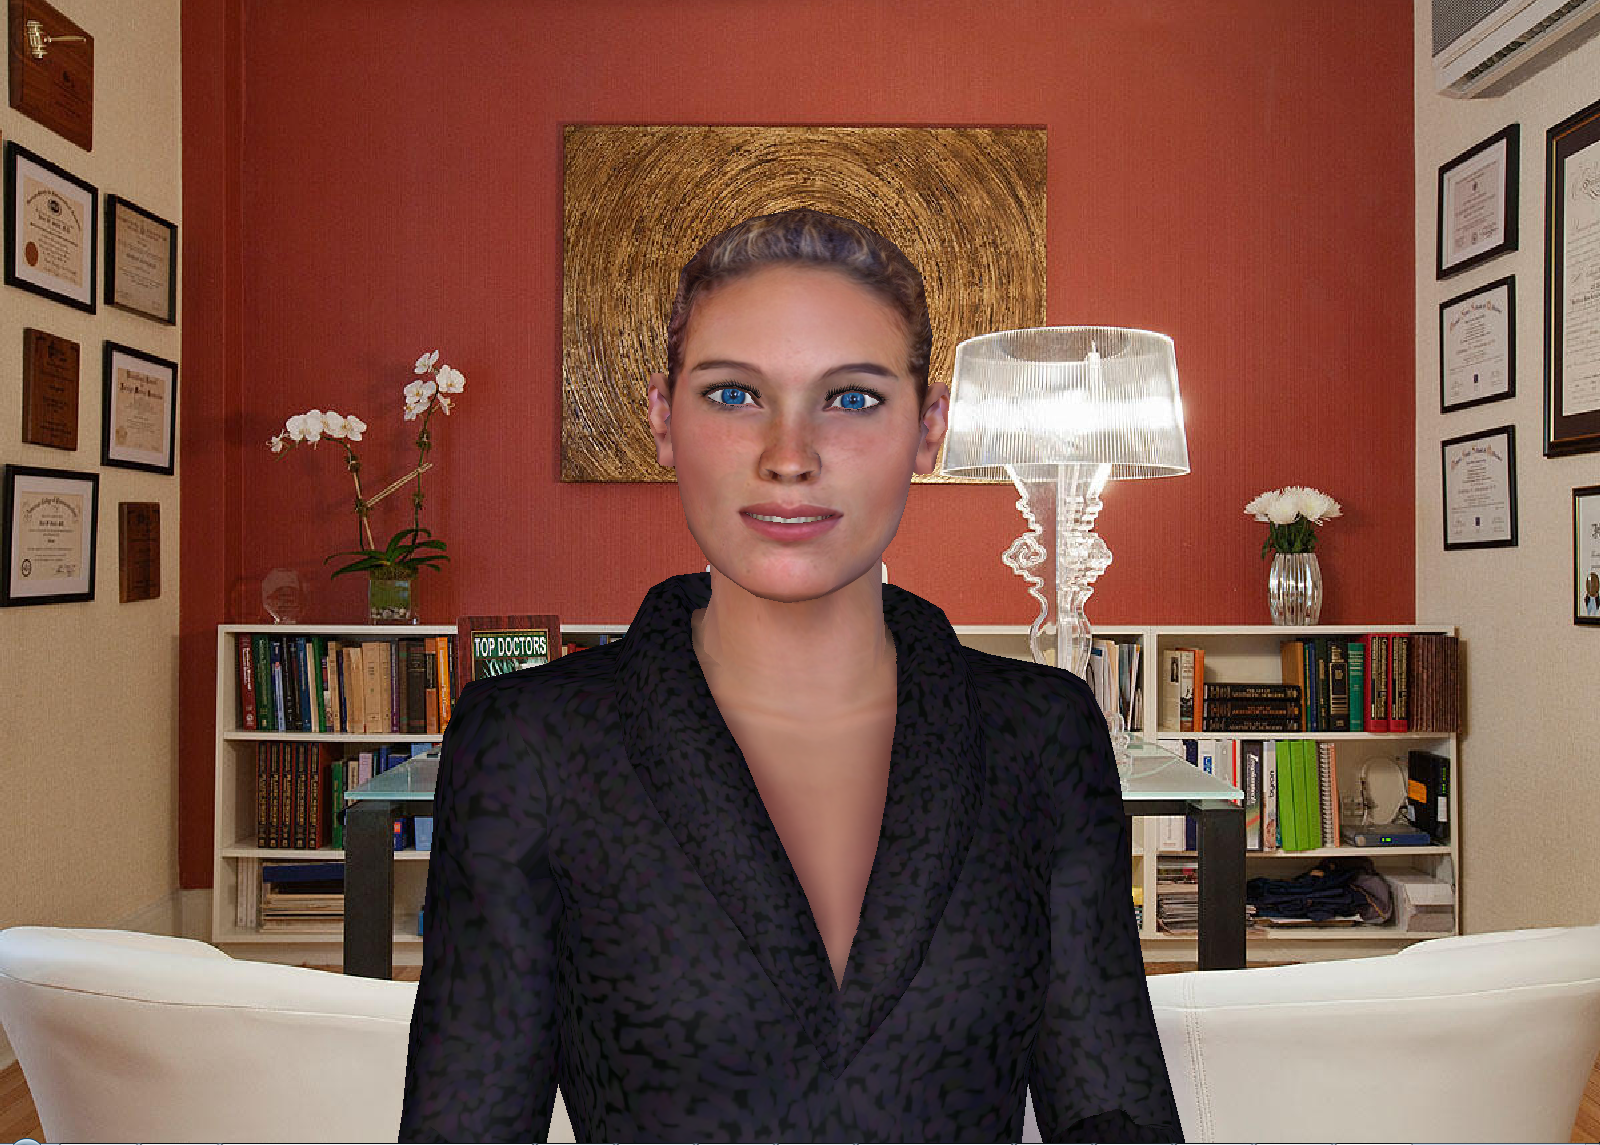
\includegraphics[width=0.48\textwidth]{img/lola.png}
% figure caption is below the figure
%\caption{Multimodal Embodied Conversational Agent Interface}
%\label{lola}       % Give a unique label
%\end{figure*}

% For one-column wide figures use
%\begin{figure}
% Use the relevant command to insert your figure file.
% For example, with the graphicx package use
%  
\includegraphics{example.eps}
% figure caption is below the figure
%\caption{Please write your figure caption here}
%\label{fig:1}       % Give a unique label
%\end{figure}
%

\begin{figure}[!t]
  \centering    
 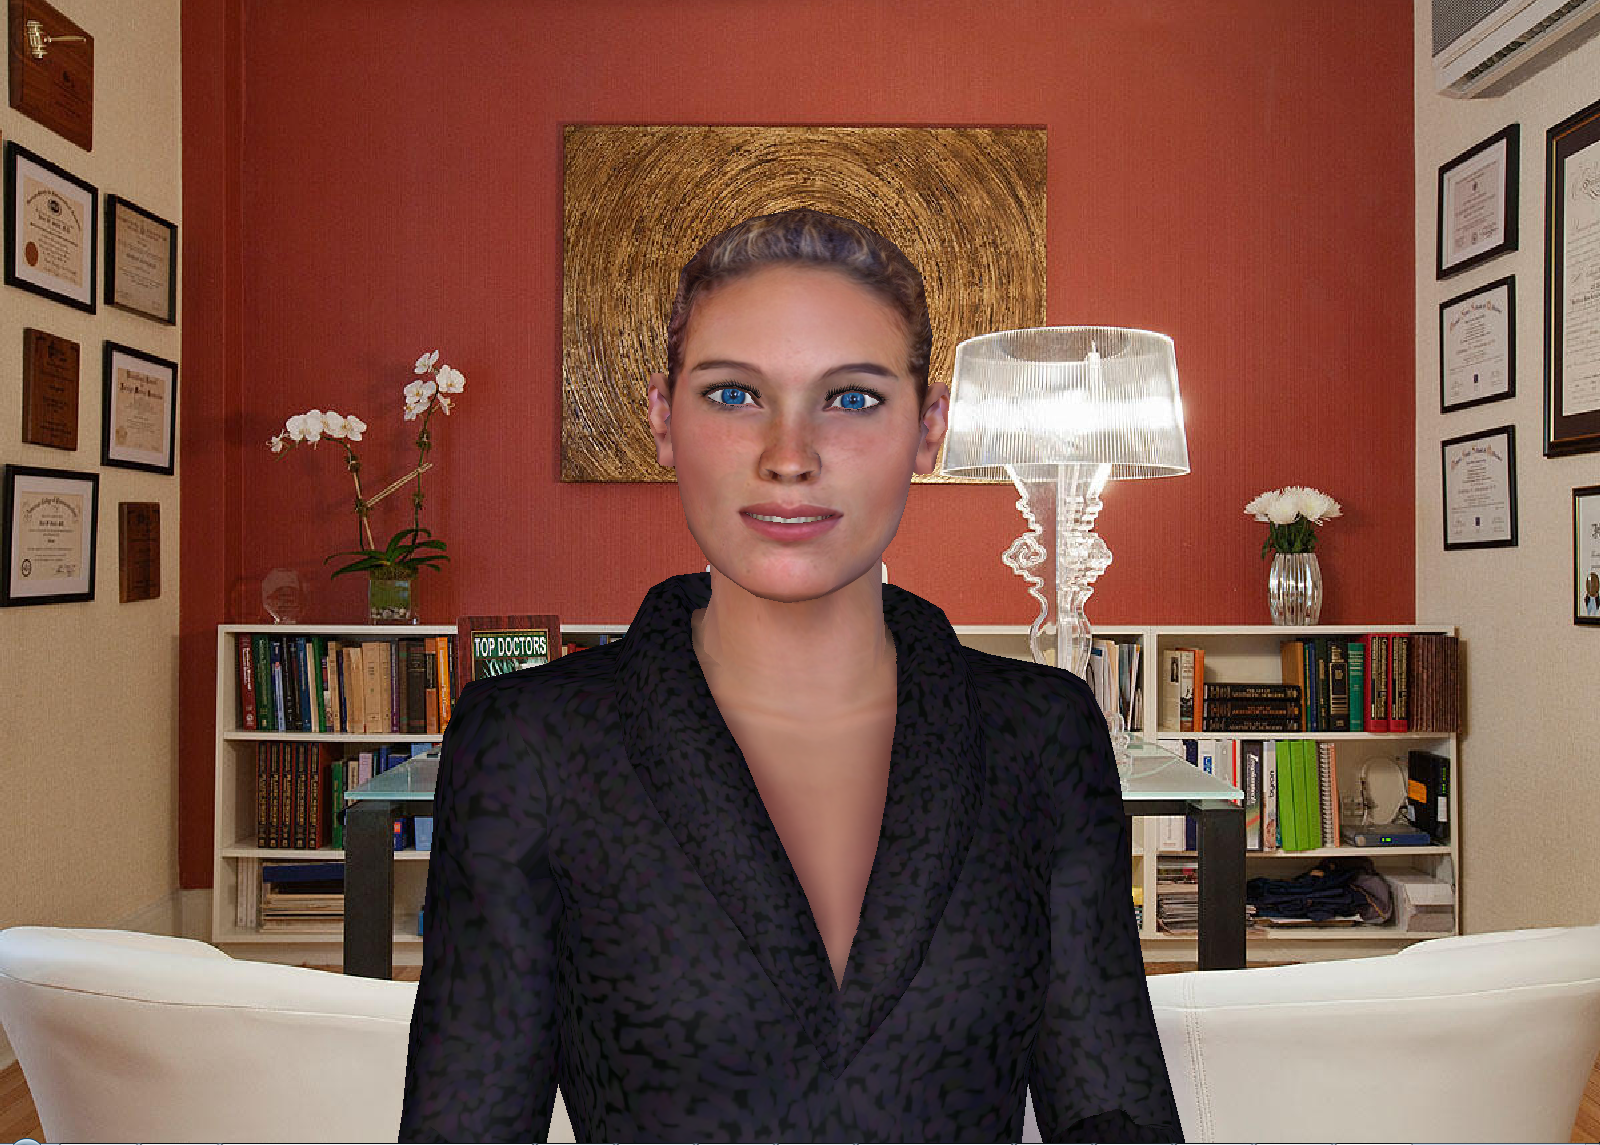
\includegraphics[width=\columnwidth]{img/lola.png}
	\caption{Multimodal Embodied Conversational Agent Interface}
  \label{lola}
\end{figure}

In this project,  we bring together latest progress from the SDS community to the IVA community with the use of RL-based dialog management integrated with a 3D animated character (shown in Figure \ref{lola}).  The 3D animated virtual character is an interface for a task-based spoken dialog to deliver brief alcohol interventions to people at-risk of health issues due to excessive alcohol consumption.  

From a computer science perspective, our work aims at building a fully implemented system to be used as screening tools to help individuals at risk of health issues, and at evaluating the system in terms of both, users' (subjective) acceptance and dialog system's (objective) performance.  

From a healthcare perspective, we aim at increasing access to effective evidence-based health interventions with a novel mode of delivery for computer-based health interventions - namely delivering health interventions with a virtual counselor.  Our screening dialog system brings insight and awareness regarding \textit{alcohol problems} by using the well established \textit{brief intervention} (BI) counseling approach.  BIs are short, well structured, one-on-one counseling sessions, focused on specific aspects of problematic lifestyle behavior.   BIs are not only ideally suited for people who drink in ways that are harmful or abusive (which is the current domain of our work), but BIs have also been used successfully for a variety of target problem behaviors (e.g. overeating, lack of exercise).  Therefore the results of our research will also have an impact on dialog systems for diverse behavior change interventions for healthy lifestyles.

In this article, we give an overview of the current brief intervention counseling style which our system is based on, as well as current progress on spoken dialog systems.  We then describe our approach to build a spoken dialog system integrated with an intelligent virtual character to deliver a brief intervention for people at-risk regarding their alcohol consumption.  We discuss the results of the evaluation of the system, and conclude with potential future directions for our field of research.


\section{Related Research}
\label{sec:RR}

\subsection{Brief Interventions for At-risk Behaviors}
\label{sec:BIs}

Excessive alcohol consumption is regarded as a very worrisome public health problem in the USA: with approximately 85,000 of directly or indirectly attributable deaths per year, excessive alcohol use is the 3rd leading lifestyle-related cause of death in the United States \cite{Mokdad2004Death}. In 2006, there were more than 1.2 million 
emergency room visits and 2.7 million physician office visits due to excessive drinking \cite{Bouchery2011}.  Excessive alcohol use is also a risk factor for many health and social problems, including motor-vehicle crashes, violence, suicide, hypertension, unsafe sex, or unintended pregnancy.  The economic costs of excessive alcohol consumption in 2006 were approximately \$223.5 billion \cite{Bouchery2011}.  To attempt to address these alarming statistics, healthcare research has led to the development and deployment of behavior change interventions that can be delivered efficiently in primary care offices.

{\em Brief interventions (BI)} are short, well structured, one-on-one counseling sessions, focused on specific aspects of problematic lifestyle behavior, and are ideally suited for people who drink in ways that are harmful or abusive. BIs can be delivered in 3-5 minutes \cite{Moyer2002} and (for alcohol consumption as a target) aim to moderate a person's alcohol consumption to reasonable levels and to eliminate harmful drinking behaviors. BIs have a  simple approach: they assess an individual's patterns of behavior with respect to a problem behavior, provide tailored feedback, and raise an individual's awareness about the problematic behavior.  BIs are the top ranked out of 87 treatment styles in terms of efficiency \cite{miller2002mesa}. It is reported that even a few minutes of discussion about behavioral problems can be as  effective as more extended counseling \cite{babor1992}.  Many challenges are involved in delivering BIs to people in need, such as finding the time to deliver them in busy doctors' offices, obtaining the extra training that helps staff become comfortable providing these interventions, and managing the cost of delivering the interventions \cite{national2006niaaa}. 

Patients are often encouraged to use computer programs developed based on BI content in the doctor's waiting room or at home, or to access the interventions through the Internet.  Computer-based interventions not only offer privacy, but also the ability to complete the program anywhere, any time of the day 
\cite{OnlineAlcoholInterventionRev2011,OnlineAlcoholInterventionRev2010,Portnoy2008}. Although computer-based interventions adapted from one-on-one brief interventions are reported to have positive effects on reducing patients' drinking level \cite{OnlineAlcoholInterventionRev2011,OnlineAlcoholInterventionRev2010,Hester2005}, they have high drop-out rates because their users loose interest with interacting with the system.  One study showed, however, that the delivery of web-based interventions with virtual agents is promising in terms of increasing people's intention to use such an intervention versus an intervention delivered with text only \cite{lisetti2013}.  That system however is not speech-enabled and the user interacts with mouse and keyboard entries. 

We posit that these challenges in administering computer-based brief interventions, can be overcome with the use of spoken dialog systems delivered by an intelligent virtual agents (or embodied conversational agent) which, integrated together, aim at emulating face-to-face conversation, which is the focus of our current research.

\subsection{Spoken Dialog Systems}

Dialog systems can be classified into two main categories based on their dialog management technique, which can be either based on machine learning (e.g. based on reinforcement learning), or hand-crafted.  Systems based on RL are popular in the SDS community and are reported to work better than hand-crafted ones for {\em speech}-enabled systems \cite{young2013pomdp,frampton2009} against noisy speech recognition. {\em Hand-crafted systems}, on the other hand, can be divided into three subcategories, with dialog management approaches using finite states \cite{sutton1998CSLU}, plans and inference rules \cite{ferguson1998trips,Bohus2009} or information states. \cite{Traum03}.

RL-based dialog systems can learn dialog strategies in a given dialog state from their prior experiences. The idea of having a dialog manager (DM) that can learn interactively from its experience is a cost effective methodology given the alternative approaches: crafting system responses to all possible user's input using rules and heuristics \cite{paek2008automating}. At best, these rules are based on accumulated knowledge from a trial-and-error experience. At worst, they are based on intuition and limited experience of the designer.  Either way, because it is extremely challenging to anticipate every possible user's input, hand-crafting dialog management strategies is an error-prone process that needs to be iteratively refined and tuned \cite{paek2008automating}.  That iterative refinement of course requires substantial amount of time and effort. 

The RL-based approach provides the opportunity to automate the design of dialog management strategies by having the system learn these strategies from received reward signals. Potential advantages of statistical dialog management approaches against hand-crafted approaches are listed by \cite{lemon2007machine} as  1) a data-driven automatic development cycle, 2) provably optimal dialog action policies, 3) a principled mathematical model for action selection, 4) possibilities for generalization to unseen states, and 5) reduced development and deployment costs.

Approaches for  dialog systems based on reinforcement learning (RL) use Markov decision processes (MDP) \cite{NjFunSingh02} or partially observable Markov decision processes (POMDP) frameworks \cite{young2010POMDP,williams2008best} to develop robust dialog managers \cite{frampton2009,young2013pomdp}. While both MDPs and POMDPs require high amount of data for training, POMDPs usually suffer from scalability issues \cite{williams2007partially,young2010hidden}, and optimization algorithms usually become intractable with large number of states. 

In this paper we used MDP approaches to avoid the mentioned problems associated with POMDPs. Unlike the classic dialog strategy learning approaches \cite{levin1998} in which the system literally has no knowledge for dialog action selection in the training stage, our system knows which actions make sense in each state,  despite being non-optimal as in \cite{NjFunSingh02}. For example, taking a farewell action at the beginning of a dialog instead of greeting does not make sense. Our approach enables our system to learn dialog strategies faster from a small amount of dialog corpus than systems with absolutely no knowledge in the training stage. 
The ideas that are used in \cite{NjFunSingh02} inspired our system design decisions: as in the NjFun system \cite{NjFunSingh02}, we tried to minimize the state space, and to learn dialog policies from real and small amount of data. We extended and adapted some of these ideas, such as state representations and policy design, and applied them to practical health applications.

RL-based dialog systems are mainly used for slot-filling applications. The domain of the dialog is usually in the tourist information domain, such as finding information about restaurants \cite{jurvcivcek2012reinforcement,Chandramohan2010,young2010POMDP}, appointment scheduling \cite{Georgila2010}, flight reservation \cite{henderson2008hybrid}, or museum guidance \cite{Papangelis2012}. There has also been work conducted in question-answering \cite{misu2012reinforcement} and tutoring domains \cite{chi2010micro}. The RL-based dialog management paradigm  was also recently used for assistive technologies  \cite{liAssistivePomdp2013}. 

In the mentioned systems, each piece of information is accepted as a {\em slot} which needs to be filled to complete the task. The total number of slots that current systems can usually handle are less than 5, and the flow of a dialog is determined by the slots that  need to be filled \cite{NjFunSingh02}.  One of the important measures of success of task-based dialogs is their {\em task completion rate}. When the number of the slots that are needed to be filled increases, the likelihood of successful completion decreases.

We will discuss how our system can handle a substantially larger number of slots than has been attempted so far (we have 18 slots).  We will also explain how the flow  of the dialog does not depend on unfilled slots, but is rather decided dynamically during the interaction, which is also a novel approach.
For example, if our system finds out that the person does not have a drinking problem, it just ends the interaction gracefully. Hence, the  length (in terms of slots) and the flow of the dialog are not fixed.

Dialog strategy learning is the main concentration of RL-based dialog systems for the optimization process. Learning optimal dialog strategies can be performed in two ways: based on user simulations \cite{georgila2006user}, or based on interactions with real users in exploration mode \cite{NjFunSingh02,misu2012reinforcement}. Since there is no data in our domain, we had to follow the latter way. It is worth mentioning that simulated users can have some shortcomings to realistically reproduce the behaviors of the diverse  real users' behaviors \cite{schatzmann2005quantitative}. 

\subsection{Assistance Technologies for Health Related dialogs}

In a recent comprehensive literature review of active assistance technologies in health-related behavior change systems \cite{kennedy2012active}, covering articles written between January 2005 and January 2012, 41 health-behavior change systems are identified. Dialog systems and ECAs are identified as emerging technology themes in the behavior change systems field. It is reported that 19 studies out of 41 use dialog systems technology. Among those 19 systems, only 1 system uses speech as an input modality \cite{Levin2006Spoken}. The remaining 19 dialog-based systems use text or menu-based choices as a style of communication. In the same literature review \cite{kennedy2012active}, it is reported that 8 of the systems use ECAs \cite{Bickmore2005,Bickmore2011,Turunen2011,DeRosis2006}.

There are also dialog systems in other health-related domains such as health and fitness companions \cite{Turunen2011}, or  virtual support agents for post traumatic stress disorder \cite{Morbini2012}. Although, there has been growing interest to develop multimodal SDS which can converse, guide, assist or motivate users for different health related topics \cite{Bickmore2011,Ferguson2010,Morbini2012}, to the best of our knowledge, there does not exist any spoken dialog system for the alcohol consumption domain, which is the focus of our research.

Furthermore, dialog management for health-related dialog systems have so far been mostly designed based on {\em finite state} dialog management mechanisms such as hierarchical transition networks \cite{Bickmore2011,Bickmore2010a}, plan-based approaches \cite{Schulman2011}, or information-state based approaches \cite{Morbini2012}.  These systems usually do not have speech recognition integration. Interaction is usually conducted with menu-based choices, but the system utterances are delivered vocally via text-to-speech or prerecorded voice \cite{lisetti2013,Bickmore2011}.  

Other than systems that use menu-based interaction, there are systems that use a different input modality. SimCoach, for example, is a web-based system which uses text as input modality, and an interface with an anthropomorphic ECA which responds to users' questions with answers prerecorded by a human.  Whereas human voices are still superior to synthetic ones, using pre-recorded utterances means that the sentences that the system can speak are fixed, as opposed to systems using text-to-speech engines (like ours) which provides the flexibility of adding new  sentences for the system to utter automatically, i.e. without the need to prerecord new sentences.  SimCoach, designed to provide support and health-care information about post-traumatic stress disorder, incorporates information-state approach \cite{Traum03} with dialog moves with assigned reward values \cite{Morbini2012}. The Companions project includes three different systems in the domain of health and fitness \cite{Turunen2011}, and all of them use speech as input modality.  The dialog management approach in the Companion project is the information-state approach, and one system (the cooking companion) has an ECA interface.

In the remaining of the article, we discuss our system design and approach, and our evaluation experiment results.  

\section{Approach}

An overview of our system architecture is shown in Figure \ref{SysArch}, and explained in details in the Section \ref{Agent}.  In short, we use reinforcement learning for the dialog management, combined with a 3D animated character who converses with the user with Text-To-Speech (TTS) utterances (versus fixed prerecorded sentences). The domain is a task-based spoken dialog to deliver brief alcohol interventions to people, and identify whether they are at-risk of health issues due to excessive alcohol consumption.  

\subsection{Dialog Structure for Brief Interventions }
\label{BIInteraction}

According to the clinician's guide for conducting brief interventions from the National Institute on Alcohol Abuse and Alcoholism (NIAAA) \cite{national2007helping}, a brief intervention for alcohol-related health problems can be delivered in three sequential steps:

\begin{itemize}
\item Step 1: {\em Screening} about alcohol {\em use}
%\vspace{}
\item Step 2: {\em Assessing} for alcohol use {\em disorders}
\begin{itemize}
%\vspace{}
\item Assessment of {\em abuse}
\item Assessment of {\em dependence}
\end{itemize}
%\vspace{}

\item Step 3: {\em Advising} and assisting according to degree of alcohol problem
\begin{itemize}
\item Advice for {\em at-risk} drinkers 
\item Advice for drinkers with alcohol use {\em disorder} 
\end{itemize}
\end{itemize}

To develop our dialog content, we follow the brief intervention guide for alcohol prepared by NIAAA \cite{national2006niaaa}. 
The goal of our dialog system is to deliver alcohol screening and brief interventions based on this guide. Each step contains a set of questions. 

In {\em Step 1}, there are 5 questions.  The system asks these 5 questions, and if the user expresses that s/he is not consuming alcohol from time to time, the interaction is gracefully terminated by the system. Otherwise, the dialog manager continues to the second step.  

In {\em Step 2}, in the Assessment of {\em abuse} stage, there are 4 questions to assess alcohol abuse indicators.  It is enough to find one indicator of alcohol abuse (e.g. risk of bodily harm, relationship trouble) to move to the Assessment of {\em dependence} stage (e.g. keep drinking despite problems, not able to stick to drinking limits). If the system can not find any indicator of abuse with the 4 questions, it passes to the dependence stage. In the Assessment of {\em dependence} stage (still in {\em Step 2}), there are 7 questions. 

It is enough to detect 3 dependence indicators to transit to {\em Step 3}, Advice for drinkers with alcohol use {\em disorder}.  If the system does not detects 3 dependence indicators, it transits to Advice for {\em at-risk} drinkers. Therefore, the dialog branches to two separate steps in {\em Step 3}: \textbf{1)} one for {\em at-risk} drinkers, and \textbf{2)} one for drinkers with alcohol use {\em disorder}. In both branches, the system provides information related to the assessment of the system.  If the system assessed that the user has an alcohol use disorder, it refers the user to treatment, asks the user if she or he is ready to change, and suggests a goal toward a change of drinking patters, based on the user's readiness. If the user is an at-risk drinker, it gauges his or her readiness to change, and provides feedback and information about the person's drinking. Therefore in both stages, the system provides factual information about the person's drinking and suggested drinking limits, and asks what is the user's intention to change with a single question.  In total there can be a maximum of 18 different questions in a single session.   

A sample dialog between the system and the user is shown in Table \ref{sampleDialog}. The dialog we presented in the table covers {em Step 1}  Screening about alcohol {\em use},  and {\em Step 2} Assessment of {\em abuse} completely. In {\em Step 2} Assessment of {\em dependence}, there are 7 questions, and then the system branches to Step 3. Because of space limitations, we cannot present a longer dialog.  The system uses questions recommended by NIAAA. It uses simple reflections for confirmations instead of explicit confirmations, and examples are shown in Table \ref{sampleDialog} with the S4 and S10 system dialog turns.


\subsection{Reinforcement Learning}

We built our system using reinforcement learning.
{\em Reinforcement Learning} (RL, henceforth) is a sequential decision making algorithm, where the RL agent interacts with its environment \cite{sutton1998reinforcement}. The environment is defined as: ``anything that cannot be changed arbitrarily by the agent is considered to be outside of it and thus part of its environment" \cite[p. 53] {sutton1998reinforcement}.  Reinforcement learning treats the learning of dialog strategies as a sequential optimization problem, leading to strategies which are globally optimal \cite{sutton1998reinforcement}. 

Within the RL framework for dialog development, dialog strategies are represented as mappings from states to actions within Markov decision processes (MDP). In other words, a dialog strategy specifies, for each system state, what is the next action to be taken by the system \cite{levin1998}. The MDP framework can be characterized by a 4-tuple (S,A,T,R), where:
\begin{itemize}
\item S is a finite set of states
\item A is a finite set of actions
\item T is a state-transition function such that \textit{T(s, a, s\textprime) = {\bf P}(s\textprime $\vert$ s, a)} which describes how the probability of performing action \textbf{a} in state \textbf{s} will lead to state \textbf{s\textprime}
\item {\bf R}(s, a, s\textprime) is a local reward function such that $ R(s, a)=\sum_a {\bf P}(a \vert s){\bf R}(s, a, s\textprime) $, and the objective of the SDS is to maximize the gained reward.
\end{itemize}



\subsection{Markov Decision Processes}

To develop our system, we needed to represent the internal states of our system using MDP formalization as described  earlier. States, actions and state transitions needed to be created. First, we elicited the state attributes. We considered the most important dialog attributes to represent the dialog state concisely. To avoid the data sparsity problem during training, we divided the whole system into 5 sections according to the BI guide steps. Hence, there are 5 MDPs in our system. For each step, we elicited related state features. 

For each state, there are 5 common {\bf attributes}: Question, Confidence, Value, Grammar, and Aux (see Table \ref{Features} for the descriptions of each attribute). There is usually 1 extra attribute to represent the step-specific requirement at each step, e.g. Greet because in the first step the system needs to greet the user first and get consent of the user to start the dialog. The full list of state features for {\em Step 1} are listed in Table \ref{Features}. 

We then designed possible {\bf states}: for each question, there are 34 possible states. 
For {\em Step 1 Use}, {\em Step 2 Abuse}, {\em Step 2 Dependence}, {\em Step 3 At-risk}, and {\em Step 3 Disorders}, the number of states are 170, 136, 238, 68 and 68 respectively, i.e. 34 states multiplied by the number of questions in a step). Total number of states is 680.
Each state represents the state of the conversation. 

For example, dialog state \textit{112101} indicates that the system has greeted the user (G=1), the first question has been queried (Q=1), the automatic speech recognizer (ASR) confidence level is high (C=2), the answer value has been obtained (V=1), the type of grammar is restrictive (Gr=0), and that the polarity of the alcohol usage indicator is positive (Ax=1). 

\onecolumn

\begin{table}
\caption{Sample Dialog}
\label{sampleDialog}
\begin{tabular}{ | l | p{13.5cm} | p{19mm} |}
\hline
S1: & Hi, My name is Lola,  I am a virtual character created to have conversations with you and to teach you about healthy lifestyles. Today, I'm here to talk about drinking to figure out if you have any issues.  May I ask you few questions about your drinking? &     \\
    C1: & Yes, sure you can. &  \\
    S2: & Do you sometimes drink beer, wine, or other alcoholic beverages? &     \\ 
    C2: & Well yes, I drink wine or beer sometimes! &    \\ 
    S3: & How many times in the past year have you had 5 or more drinks in a day? &  \\ 
	C3: & I think around once a week. &    \\ 
	S4: & Actually, consuming more than 4 drinks on any single day is classified as heavy drinking. So it seems that you are sometimes going above heavy drinking limits? Is that right? &  \\
	C4: & Yes, that's correct. & \\
	S5: &  How frequently do you have an alcoholic beverage each week? &    {\em Step 1}:   \\ 
	C5: & I think at least 3 days a week.  &  {\em Use} Screening \\ 
	S6: & On a typical drinking day, how many drinks you have? &    \\ 
	C6: & I just drink... maybe a bottle of whisky. &    \\ 
	S7: & Sorry, I could not understand your answer, can you please repeat? & \\
	C7: & I said one bottle of scotch. & \\
	S8: & Ok, thanks for the information you have provided to me about your drinking. Next, I will try to determine some important effects of your drinking. &  \\ \hline
	S9: & Have you ever taken risks under the influence, such as drinking and driving, operating a motor vehicle, or swimming? &    \\
	C9: & No I have not. &  \\
	S10: & I see, so you are careful to avoid high risk situations after or while having drinks, right? & \\
	C10: & Yes, I try to be careful. &  {\em Step 2}: {\em Abuse}   \\
	S11: & Have you continued to drink even though you knew it was causing you trouble with your family or friends? & Assessment \\
	C11: & I think yes, I continue to drink while my family complains about my drinking. & \\
	S12: & Thanks for the information you've provided. In the next step, I will ask you questions about potential dependence-related aspects of your drinking. Is that okay? & \\
	C12: & Yes I want to know, please go ahead. & \\
	 \hline
	S13: & Have you had times when you ended up drinking more than you meant to? Or kept on drinking for longer than you intended? &  \\ 
	C13: & Not usually, but... yes I guess I did. & \\
	S14: & Have you found that you have to drink much more than you once did in order to get the effect that you like? & \\
	C14: & I think my tolerance has increased. & \\
	S15: & Sorry, I could not understand your answer. Do you need to drink a lot more sometimes to get the same effect? & \\
	C15: & I meant yes, I need to drink more and more. &\\
	S16: & Ok, sorry but just be sure I got it right: you can not get the same effect as you used to with the same amount of alcohol. Is that right? & \\
	C16: & Yes, that is correct. & \\
	S17: & Have you more than once wanted to stop or cut down on your drinking? Or tried more than once to stop or cut 
	down but found you couldn't? & \\
	C17: & Well, I think I tried but I was not that serious about stopping or cutting down. & Step 2:  \\
	S18: & I see, so you really never attempted to stop or cut down. Is that right? & {\em  Dependence} \\
	C18: & No, it is wrong. &  Assessment \\
	S19: & Sorry for the misunderstanding, can you please repeat your answer? Have you more than once wanted to stop or cut down on 
	your drinking but found you couldn't? & \\ 
	C19: & Yes I did but not seriously. & \\
	S20: & Ok, now, when the effects of alcohol are wearing off, have you had trouble sleeping, or found yourself shaking, nervous, nauseous, or restless?  & \\
	C20: & I found myself sweating and my heart beating fast. & \\
	S21: & Sorry I could not understand your answer. Can you please repeat it? & \\
	C22: & I said I found myself sweating and my heart beating fast. & \\ 
	S22: & I am sorry for asking again, but can you repeat your answer please? & \\
	C22: & I said I am sweating and my heart beats fast when I drink too much. & \\
	S23: & Have you had a period when you spent a lot of time drinking? Or being sick or getting over the bad aftereffects of drinking? & \\
	C23: & Yes several times. & \\
	\hline
	S24: & Thank you very much for all your answers. Now I'd like to just take one or two more minutes of your time. Is that okay? &\\
	C24: & Yes, please go ahead. & \\
	S25: & On a scale from 1 to 10, how ready are you to make a change? & \\ 
	C25: & I think 7. & {\em Step 3}:  \\
	S26: & Great! Just for your information,  men who drink more than 4 standard drinks in a day or more than 14 per week, and  women  who drink more than 3 drinks in a day or more than 7 drinks per week, are at increased risk of  alcohol related problems. Based on your answers, I recommend that you stick with this limit, or even abstain if you can.  I also would like you to track your drinking patterns, and I could send you a calendar for that if you'd like me to. I'm also going to give you information about places near you where you can get help if you choose to.  Finally, I would like to talk with you again in 3 months. Is that okay? & {\em Disorder} \\
	S26: & Yes, it's okay. & \\
	S27: & Thanks for talking with me. I hope you've learned something useful about your drinking pattern.  Good bye and let's talk again in 3 months! & \\
 	\hline
    \end{tabular}
   \end{table}

\twocolumn

 An alcohol usage indicator is positive if consuming alcoholic beverages is above recommended limits, and negative if consumption is below limits. The Aux attribute is used for multiple purposes, such as keeping track of the number of re-asked questions, or of the polarity of alcohol problem indicator. Aux is set to 0 when it is not used.

\begin{table}[h]

\caption{State attributes and values for {\em Step 1}: Screening About Alcohol {\em Use}}
\label{Features}
\tabcolsep1mm
\begin{tabular}{ | p{20mm} | p{10mm} | p{47mm} | } \hline
    \textbf{Attribute} & \textbf{Values} & \textbf{Description} \\
    \hline
    Greet (G) & 0,1 & Whether the system has greeted the user \\
    \hline
    Question (Q) & 1,2,3,4 & Which question is being queried \\
    \hline
    Confidence (C) & 0,1,2,3, 4,5,6 & 0,1,2 for low, medium, and high confidence of speech recognizer. 3,4 for confirmed or not confirmed. 5 to indicate system is waiting for confirmation. 6 is for to indicate system transit to next question without confirmation \\
    \hline
  Value (V) & 0,1 & Is the value obtained for current question \\
  \hline
  Grammar (Gr) & 0,1 & What type of ASR grammar used, restrictive or dictation (non-restrictive) grammar.  \\
    \hline
      Aux (Ax) & 0,1,2 & Multiple purpose attribute. Use to indicate number of ReAsks and semantic valence of the received answer. If it is 0, it indicates, it is not used in that state.  \\
        \hline
\end{tabular}
\end{table}

\begin{table*}[t]
\caption{Dialog Actions For Question1 in Step 1}
\label{dialogActions}    
\begin{tabular}{ | l | p{130mm} |}
    \hline
	{\bf Dialog Action} & {\bf System Utterance} \\
	\hline
	S1-AskQ1Sys: & Do you sometimes drink beer, wine, or other alcoholic beverages? \\
	S1-AskQ1User: & Can you briefly talk about your alcohol consumption? \\
	\hline
    S1-ReAskQ1Sys & Sorry, I could not understand your answer. Do you sometimes drink beer, wine, or other alcoholic beverages? \\
    S1-RaAskQ1User: & Sorry, I could not understand your answer. Can you briefly talk about your alcohol consumption? \\
\hline
S1-ConfQ1Pos & So you like to have alcoholic beverages from time to time, is that right? \\
S1-ConfQ1Neg & So you are recently not having any alcoholic beverages, is that right? \\
S1-NoConf & --- \\
\hline
	S1-NotConfirmedQ1Sys & I am sorry for the misunderstanding.  Do you sometimes drink beer, wine, or other alcoholic beverages? \\
		S1-NotConfirmedQ1User & I am sorry for the misunderstanding, can you briefly talk about your alcohol consumption? \\
 	\hline
    \end{tabular}
 % \begin{tabnote}
%     \Note{The first column contains dialog action name. The second column is the corresponding utterance for the dialog action.}
%     \end{tabnote}
   \end{table*}


  We refined our state representations by excluding the states that make no sense and manually checking each state. For example, state \textit{040111} is a non-sensible state in {\em Step 1}. The system can not be in that state because the system needs to greet the user {\em first}, before it can ask questions. It is not possible to ask question 4 in the first step without greeting or without asking prior questions. Excluding non-sensible states yielded a very large state-space reduction.

We then created our {\bf dialog actions} for each question. Our system uses 2 types of initiative dialog actions: system initiative, where the system asks close-ended questions (e.g. Do you sometimes drink beer, wine, or other alcoholic beverages?), and user initiative, where the system asks open-ended questions (e.g. Can you briefly talk about your alcohol consumption?). We refer to the system/user initiative terms in the same manner as they are widely referred to in the SDS community \cite{NjFunSingh02,singh2000empirical}.  In the system initiative questions (where the expected answer is relatively restricted given the close-ended nature of the questions), the system uses a restrictive grammar for speech recognition (SR).  In the user initiative, the system uses a non-restrictive SR grammar to handle user's answer to open-ended questions. 

There are 9 possible actions for each question, which are grouped under 4 categories: \textbf{1)} \textit{Ask} actions are used when the system needs to ask a question to the user for the first time, which can be performed with the two types of initiatives; \textbf{2)} \textit{ReAsk} actions are used if the system can not understand the user's speech, which can also be done with two types of initiatives; \textbf{3)} \textit{Confirmation} actions are used to ask for confirmation as to whether the system understood what the user said. 

The confirmation actions are system initiated by default, and are of 3 types: positive, negative and no confirmation. The positive type is used if the system receives an answer which reveals alcohol usage/abuse/dependence information. The negative type is used if the system receives an answer which indicates no drinking/abuse/dependence problem. The third type is no-confirmation, and it is used if the system decides to pass to the next question without confirmation (possible action at any question). \textit{NotConfirmed} action is used if the user gives a negative answer to a confirmation action. 

The available actions for the first question in \textit{Step 1} Screening About Alcohol {\em Use} are shown in Table \ref{dialogActions}. The first column is the name of the dialog action, and the second column is the system utterance. The actual name of the dialog action starts with the step information (e.g. S1), then the type of dialog action (e.g. Ask), then the question being queried (Q1) and the initiative type (Sys). So S1-AskQ1Sys stands for \textit{Step1} (S1), the question type is \textit{Ask}, the question being queried is \textit{question one} (Q1) and the initiative type is \textit{system initiative} (Sys).

The number of available actions for each question is 9 (as for the first question shown in Table \ref{dialogActions}). Although the length of the dialog is not fixed, our system asks a maximum of 18 questions. There are 162 available actions (for asking questions, re-asking questions, and confirmations) for the system to select from in the  longest dialog session (18 questions multiplied by the number of available actions). There are dialog actions which are used while transiting from one step to another step (e.g. from {\em Step 1} to {\em Step 2 Abuse}) and dialog actions for ending the conversation.  There are 2 actions for giving feedback to at-risk drinkers and to drinkers with alcohol use disorder at the end of the each session. The total number of the dialog actions is 169.

\begin{table} 
\tabcolsep1mm
\caption{Explaratory Policies For Step 1 Question 1}
\label{PolicyTable}
\begin{tabular}{ | l l l l l l | p{49mm}| } \hline
    \multicolumn{6}{|l|}{\bf States} & {\bf Available Actions per State} \\
    \textbf{G} & \textbf{Q} & \textbf{C} & \textbf{V} & \textbf{Gr} & \textbf{Ax} & \\
    \hline
   1 & 1 & 0 & 0 & 0 & 0 & S1-ReAskQ1Sys, S1-ReAskQ1User \\
   1 & 1 & 0 & 0 & 1 & 0 & S1-ReAskQ1Sys, S1-ReAskQ1User \\
   1 & 1 & 0 & 0 & 0 & 1 & S1-ReAskQ1Sys, S1-ReAskQ1User \\
   1 & 1 & 0 & 0 & 0 & 2 & S1-AskQ2Sys, S1-AskQ2User \\
   1 & 1 & 0 & 0 & 1 & 1 & S1-ReAskQ1Sys, S1-ReAskQ1User \\
   1 & 1 & 0 & 0 & 1 & 2 & S1-AskQ2Sys, S1-AskQ2User \\
   1 & 1 & 0 & 1 & 0 & 1 & S1-ConfQ1Pos, S1-NoConf \\
   1 & 1 & 1 & 1 & 0 & 1 & S1-ConfQ1Pos, S1-NoConf \\
   1 & 1 & 2 & 1 & 0 & 1 & S1-ConfQ1Pos, S1-NoConf \\
   1 & 1 & 0 & 1 & 1 & 1 & S1-ConfQ1Pos, S1-NoConf \\
   1 & 1 & 1 & 1 & 1 & 1 & S1-ConfQ1Pos, S1-NoConf \\
   1 & 1 & 2 & 1 & 1 & 1 & S1-ConfQ1Pos, S1-NoConf \\
   1 & 1 & 0 & 1 & 0 & 2 & S1-ConfQ1Neg, S1-NoConf \\
   1 & 1 & 1 & 1 & 0 & 2 & S1-ConfQ1Neg, S1-NoConf \\
   1 & 1 & 2 & 1 & 0 & 2 & S1-ConfQ1Neg, S1-NoConf \\
   1 & 1 & 0 & 1 & 1 & 2 & S1-ConfQ1Neg, S1-NoConf \\
   1 & 1 & 1 & 1 & 1 & 2 & S1-ConfQ1Neg, S1-NoConf \\
   1 & 1 & 2 & 1 & 1 & 2 & S1-ConfQ1Neg, S1-NoConf \\
   1 & 1 & 6 & 1 & 1 & 1 & S1-AskQ2Sys, S1-AskQ2User \\
   1 & 1 & 6 & 1 & 1 & 2 & S1-Q1End, S1-Q1End \\
   1 & 1 & 6 & 1 & 0 & 1 & S1-AskQ2Sys, S1-AskQ2User \\
   1 & 1 & 6 & 1 & 0 & 2 & S1-Q1End, S1-Q1End \\
   1 & 1 & 3 & 1 & 0 & 1 & S1-AskQ2Sys, S1-AskQ2User \\
   1 & 1 & 3 & 1 & 1 & 1 & S1-AskQ2Sys, S1-AskQ2User \\
   1 & 1 & 3 & 1 & 0 & 2 & S1-Q1End, S1-Q1End \\
   1 & 1 & 3 & 1 & 1 & 2 & S1-Q1End, S1-Q1End \\
   1 & 1 & 4 & 1 & 0 & 1 & S1-NotConfirmedQ1Sys,S1-NotConfirmedQ1User \\
   1 & 1 & 4 & 1 & 1 & 1 & S1-NotConfirmedQ1Sys,S1-NotConfirmedQ1User \\
   1 & 1 & 4 & 1 & 0 & 2 & S1-NotConfirmedQ1Sys,S1-NotConfirmedQ1User \\
     1 & 1 & 4 & 1 & 1 & 2 & S1-NotConfirmedQ1Sys,S1-NotConfirmedQ1User \\
 	  \hline
         \end{tabular}
%   		\begin{tabnote}
%   		     \Note{Explaratory Policy Table, first column shows states and second column is showing the available actions for each state. State features are given in Table \ref{Features}}
%   		     \end{tabnote} 		 
\end{table}


After creating the dialog actions, we created the {\bf dialog policies}. A dialog policy is a mapping of a state to sensible dialog actions. We mapped each state to 2 possible dialog actions based on the initiative or confirmation type. Table \ref{PolicyTable} shows exploratory dialog policies for  Question 1 in Step 1. 



\begin{figure*}[t]
  \centering    
	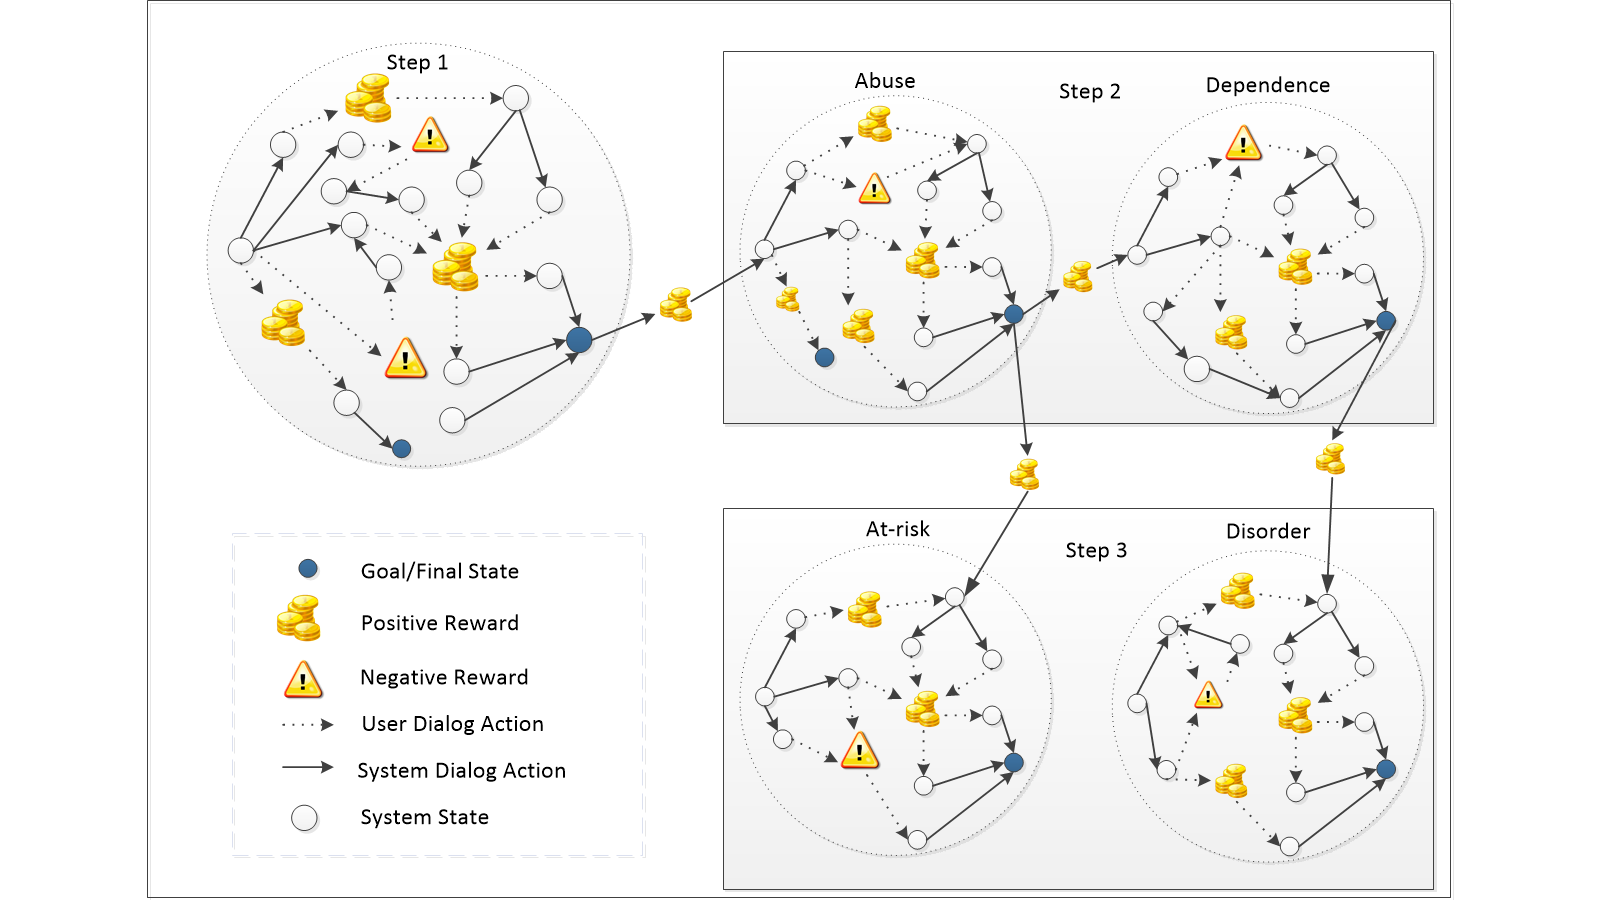
\includegraphics[scale=0.37]{img/5MDPV2.png}
	\caption{Representation Of World Model With MDPs}
  \label{5mdp}
\end{figure*}



As we mentioned earlier, for each question there are 34 states. State updates are performed based on user's dialog actions or on systems dialog actions in each dialog turn. In Table \ref{PolicyTable}, only 30 state-actions mappings that are updated by the system dialog actions or user dialog actions are shown. The remaining 4 states are only updated based on user's dialog actions, which is why we did not include them in Table \ref{PolicyTable}. The reason for this is that, if the system waits for the confirmation from the user (i.e. where C=5 as shown in see Table \ref{Features}), the system dialog actions can not be used to update a state. In other words, the remaining 4 states need to be updated by user's dialog actions. In Table \ref{PolicyTable}, we only show the states that are updated by the system. However, the states in Table \ref{PolicyTable} are the result of the user's dialog actions since \textit{Value Grammar, Confidence} and sometimes \textit{Aux} are updated by user's dialog actions in each dialog turn. For example, when the user speaks to the system, the speech recognizer \textit{Confidence} level and \textit{Value} attributes are updated based on the user's dialog action. Our system aims to learn approximately optimal dialog strategies for the initiative style and the confirmation type selection.

\subsection{Modeling World with Interconnected MDPs}

To avoid the curse of dimensionality problem, we aimed at minimizing the number of system states used. Since the BI dialog requires many dialog turns between the system and a user, the number of available dialog strategies is very large, and can make learning optimal policies infeasible with limited training data. To alleviate this problem, we used separate MDPs for each phase.

We represent each step or phase of the BI with one MDP with local goals and reward functions. This approach divided the problem into 5 interconnected MDPs (shown in Figure \ref{5mdp}) but, in any interaction with the system, we use a maximum 4 MDPs, i.e. 1) Step 1; 2) Abuse; 3) Dependence; and 4) one MDP from Step 3 based on Abuse or  Dependence problem. This approach also reduced the number of required state features for each step, thus reducing the number of states required. 

Since there are two phases in {\em Step 2} (one for querying alcohol abuse and one for querying alcohol dependence), we represent Step 2 with two distinct MDPs (as shown in Figure \ref{5mdp}), which greatly reduces the number of exploratory policies (because it reduces the number of state features) without compromising fine-grained distinctions between dialog strategies. Because the two phases are independent from each other, representing each phase with a separate MDP is appropriate.
 
There are two separate MDPs for representing the two different phases in {\em Step 3}.  One is used for representing the model for ``At-risk" drinkers who do not have alcohol use disorder problems (i.e. no abuse nor dependence). The second one is used to identify drinkers with alcohol use disorders.

In conclusion, the system is modeled with 5 MDPs. In each MDP, there are multiple terminal states. Some terminal  states  terminate the  Step  (such  as the  consent state), and  some terminal  states  provide  transparent transitions to  the start state  (or start state  distribution) of another MDP (see Figure \ref{5mdp}). %Each local goal state deterministically transits the dialog state to the start state of a successor MDP (see Figure \ref{5mdp}) or it ends the dialog. 
At the same time, the agent receives a positive reward. The agent also receives immediate positive/negative rewards as showed in Figure \ref{5mdp}. For details on immediate rewards, please see Section \ref{Reward}. With this approach, learning the optimal dialog strategy for an entire dialog is reduced to learning optimal dialog strategy for each of the MDPs. 


\subsection{Agent and dialog Strategy Learning}
\label{Agent}


\begin{figure*}
\centering
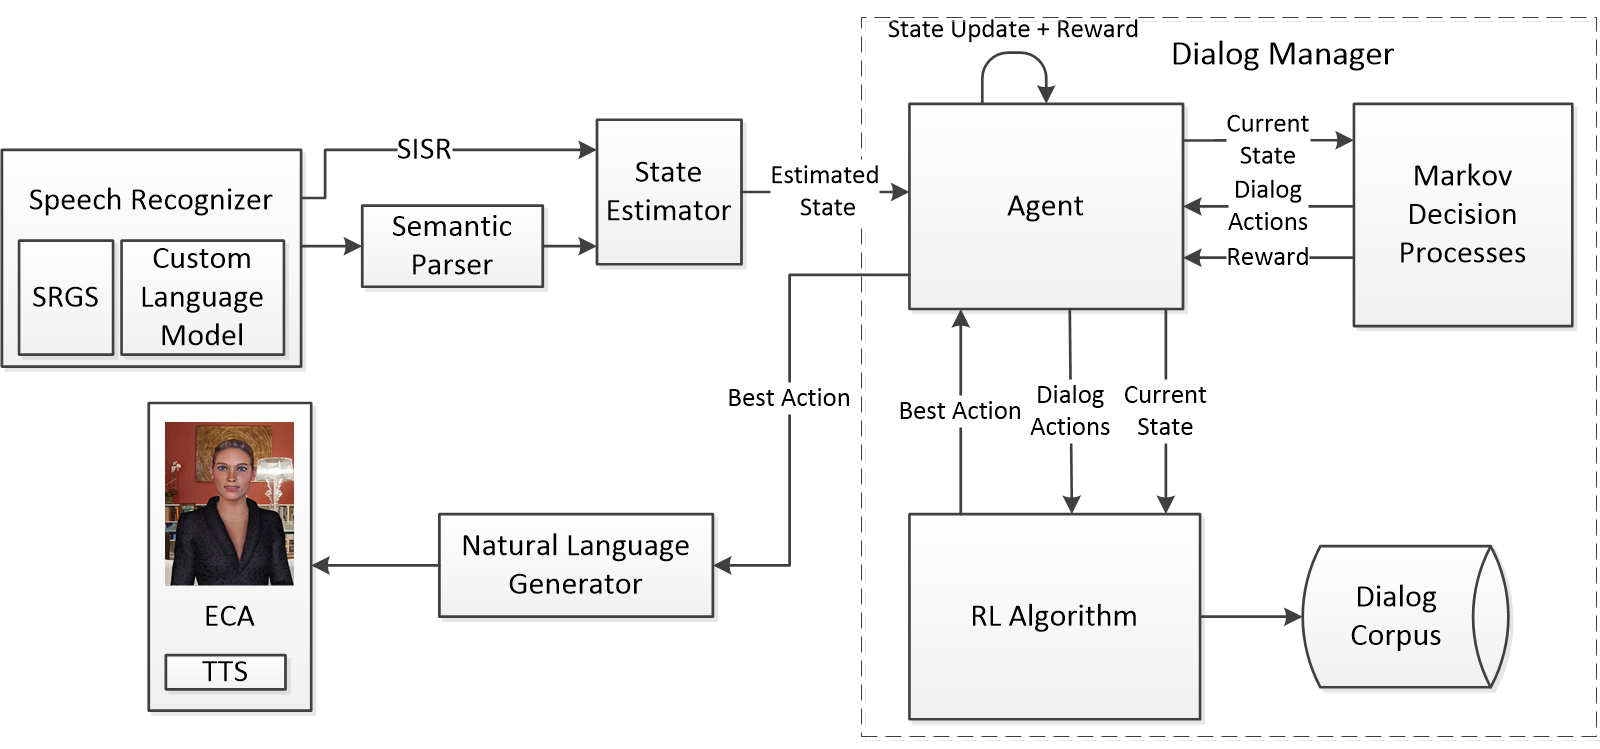
\includegraphics[height=68mm]{img/SystemArchWithStateEstimator.png}
\caption{System Architecture and dialog Manager}
\label{SysArch}
\end{figure*}

As shown in  Figure \ref{SysArch}, the {\em Agent} component of the system operates as an interface between other main components of the system. If the system asks a system initiative question, the {\em Speech Recognizer} component operates by using {\em Speech Recognizer Grammar Specification (SRGS) grammars}\footnote{http://www.w3.org/TR/speech-grammar/}, and it outputs {\em Semantic Interpretation for Speech Recognition\footnote{http://www.w3.org/TR/semantic-interpretation/} (SISR)} tags. 
If the system uses non-restrictive grammar, it uses the {\em Semantic Parser} to parse the recognized speech. We use the Phoenix robust semantic parser \cite{PhoenixParser1991}, which requires to write context-free grammar style recursive grammars to extract relevant information from the user utterances. 

Therefore the \textit{Agent} component receives SISR tags (i.e. when the type of system dialog action is system initiative or closed questions), or Phoenix  parse results (i.e. when the type of system dialog action is user initiative or open questions) according to the initiative type, as semantic interpretations. The agent updates the system {\em Current State} and collects the {\em Reward} according to the reward function (see section \ref{Reward} for the reward function). It then queries the corresponding {\em Markov Decision Process} with the current state, and receives {\em Dialog Actions} and a {\em Reward}  information for the current state, and there might not be any associated rewards.

A reward is received only if the {\em Current State} has an associated {\em Reward}. For example, the final state of each MDP has associated rewards. The agent sends the received {\em Dialog Actions} from the MDP and the {\em Current State} to the {\em RL algorithm}, and the RL algorithm selects the {\em Best Action - an action for which the agent received a maximum amount of reward in its prior experience -} based on the {\em Dialog Corpus} (see section \ref{corpus}) which is collected from real user interactions.The dialog corpus contains information about gained rewards at each step and accumulated rewards for a whole dialog session.  The best action is the one that leads the agent to collect the maximum amount of reward. If the system is running in exploration/unoptimized mode, it selects dialog actions randomly among available actions in that state. Therefore, the best action selection does not happen in the unoptimized version which is usually used to collect training data (exploration mode).

The {\em Best Action} is passed to the {\em Natural Language Generator} component, which gives the final form of the system response and passes the text to the {\em Text-to-Speech (TTS)} engine. The embodied conversational agent {\em ECA} utters the  response with lip synching.  After each dialog turn, the {\em Dialog Corpus} is updated by the {\em Agent} with the old dialog state, action, the new dialog state and the reward information. Actually, the corpus contains more information about each turn but the RL algorithm uses reward signals to select the best dialog actions in each state.


At the inception of the project, we did not have any data for optimizing the system for our domain of discourse (the domain of alcohol use). So we first used the system with an algorithm which selects a dialog action randomly among the available ones. Since we have mapped each state to sensible dialog actions, the system was able to deliver basic unoptimized functionality. 


After having acquired the {\em Dialog Corpus} for the domain of alcohol abuse - which is itself a contribution as it can be reused - we used the RL algorithm to learn optimized dialog policies and select the best action according to available data (see section \ref{experiment}).

Based on each of our MDPs, the expected cumulative reward \textit{Q(s, a)} of taking \textit{action a} from \textit{state s} can be calculated in terms of Q-values of the next dialog states with the following equation \cite{sutton1998reinforcement};


\begin{equation}
Q^*(s,a)= R(s, a) + \gamma \sum_{s'} {\bf P}(s' | s, a) \max_{a'}Q^*(s', a').
\label{equation}
\end{equation}

where ${\bf P}(s' | s, a)$ is the transition model and R(s, a) is the local reward function. The $\gamma$  $ (0 \le \gamma \le 1) $ is the discount factor which is mainly used to indicate the importance of sooner versus later rewards. 

The Q-values in Equation 1 can be easily computed with a desired threshold using the Q-value version of the standard {\em Value Iteration algorithm} \cite{sutton1998reinforcement}.  The algorithm updates iteratively the current value of Q(s, a) based on the current Q-values, and it stops when the update yields a difference that is below the threshold. Once the Value Iteration algorithm is completed, approximately optimal dialog strategies can be selected by the system, which are essentially dialog actions with the maximum Q-values. The optimized dialog strategy must collect the maximum amount of rewards from future users. 

The biggest challenge of this approach is in collecting enough human-machine dialog data to learn an accurate model. To avoid the data sparsity problem, we used minimal state representations and approximated the true state of the system during the interaction. Since the length of the dialog is long, a large amount of data is required to optimize the system. As we describe in Section \ref{experiment}, we run the systems in two modes, training/exploration and testing. Training mode is for data collection, and in testing mode, the system uses optimized dialog strategies based on the data collected in training. Therefore, Equation \ref{equation} is used only for testing mode.

\subsection{Reward Function Design}
\label{Reward}

The reward function we use is designed based on the amount of information collected and the cost of collecting each piece of information. The agent gets a reward in each question: if the value is obtained in the first attempt with the \textit{ASK} type of action, it gets +10 reward; if on the other hand the value is not obtained, the agent gets no reward. For each \textit{Confirmation} action, if the obtained value is confirmed by the user, it gets +2, otherwise it gets -2. For each \textit{ReAsk} action which could not result in obtaining the necessary information, the agent receives -3 reward, otherwise it receives +3 reward for the obtained value. If the obtained value is disapproved by the user, it deletes the previously gained reward. Therefore the agent gains a positive or negative reward for each question and dialog action. In addition to rewards gained per question, there are rewards in the MDPs which are associated with the final states. The system receives +15 reward if it is able to reach any of the final states in any MDP. For example, the successful completion of Step 1 gives the agent a +15 reward. In Figure \ref{5mdp}, we depict the immediate rewards and the rewards that are received from the goal states for each MDPs.

We have used this approach to perform strategy learning for each question. Since the system tries to obtain one piece of information in each question, learning the approximately optimal actions in each question is useful.

\subsection{Speech Recognition and Language Model}
\label{speechRecognition}

In our system, the operation mode of the speech recognizer\footnote{Microsoft Speech Recognizer} is adapted according to the dialog manager's action selection. If the dialog manager asks {\bf system initiative} questions to the user, the system uses {\em Speech Recognizer Grammar Specification (SRGS) grammars}. Even though we refer to system initiative questions as closed questions, our SRGS grammar does not restrict the user to answer with short answers such as yes/no or a number. It can still understand unrestricted speech. 
If the system operates in system initiative mode, the Phoenix parser is not used. Instead {\em Semantic Interpretation for Speech Recognition (SISR)} tags are used. We created a grammar by first authoring it in Augmented Backus-Naur Form (ABNF), and then we converted it to SRGS by using the NuEcho\footnote{http://www.nuecho.com/en/} ABNF editor. 

Our system uses our custom dictation grammar while it operates in {\bf user initiative} mode. In user initiative mode, we load two types of grammars in the in-process speech recognizer. One is the SRGS grammar which is prepared for the system initiative version of the current question. If the speech recognition result is based on dictation grammar, we use the Phoenix parser, otherwise we use SISR tags. Since the standard dictation language model is comprehensive, it does not work well in specialized domains. To address this problem, we  created our own language model by using Windows Vista Dictation Resource Kit software. It is a tool which enables the creation of custom speech recognition dictation language models. 

{\bf Language models} help a speech recognizer decide upon the likelihood of a word sequence.  Hence it is useful independently  of the acoustics of the word sequences. A language model lets the recognizer make the right guess when two different sentences sound similar.  For example, both of the following sentences sound similar: ``Because of alcohol, I had hard problems" and ``Because of alcohol, I had heart problems". With a language model on alcohol consumption, the recognizer knows that the first sentence is more likely to be what was said than the second one.  Furthermore, a language model does not only give information about homonyms, it also gives statistical information about which word might appear after another, among other information.  Therefore, if a language model consists of word sequences that are relevant in a specific context, it is very likely that it will operate better than a comprehensive language model for English.

To collect the data for the language model, we first collected data using the Mechanical Turk (MT) crowd sourcing website\footnote{https://www.mturk.com} after obtaining Internal Review Board approval for the study.  We asked MT participants the same questions that our system  in full mode would ask (after being built from the process described above and after we have acquired the language model). In the instructions, we requested them to role play a person who is having alcohol problems. Our instructions were:

 ``\textit{Imagine that you are recently having drinking problems and that you are talking with a health professional face-to-face about your drinking problems. The health practitioner asks you the questions on this page. Please answer as naturally as possible."}

Because alcohol usage is a very common and universal social problem that everyone understands, MT users' answers were relevant.  Once can note that we would not necessarily had collected meaningful answers had we asked MT users, for example, to imagine having some complex disorder such as schizophrenia, because most people do not know what behaviors are associated with this condition.  Consuming alcohol in different quantities however, is an experience that many people can relate to, and therefore the answers that we collected were very relevant.

Participants answered the 18 questions. We  created the language model from the responses of 447 MT workers. We preprocessed it (corrected  spelling and grammar problems) before creating the language model. We improved the language model by adding sentences generated based on our SRGS grammars, and used this language model in our experiments. In the model, there are 7,599 utterances, the average length of an utterance is 11.82 words, there are 100,679 word tokens, and 5,423 distinct words. 

We used our custom language model in our evaluation (see section \ref{experiment}). We collected the training data from real user dialogs (described in Section \ref{corpus}) which includes sound files. We ran the speech recognizer on the collected sound files and compared recognitions based on the two language models.  We performed quantitative analysis to compare the Microsoft standard dictation language model with our custom language model. We found that when we use our custom language model, the word error rate is approximately 17\% lower than the Microsoft standard dictation language model.
  
\subsection{Dialog Corpus}
\label{corpus}

We created a very richly annotated XML-based dialog corpus from the test dialogs, whose size will continue to grow as we collect more data. The corpus is organized turn by turn. Each turn element contains: step and state information, question asked by the system,  initiative type,  best speech recognition, grammar type, semantic value or result of the Phoenix parser, N-best recognitions with confidence score, reward gained from the question, cumulative reward and sound files. Each XML log file contains sequences of dialog turns for one dialog session. 

\section{Evaluation}

\subsection{Participants and Procedure}
University students represents a very appropriate sample for target population for brief interventions. The latest report of NIAAA on college drinking indicated that alcohol problems are very prevalent among college students \cite{NIAAA2007colleges}, and 19\% of college students (ages 18-24) meet the criteria for alcohol abuse or dependence\footnote{From the Diagnostic and Statistical Manual of Mental Disorders, Fourth Edition (DSM–IV), American Psychiatric Association.}. The use of brief interventions with college students to educate students about drinking and  increase their awareness is very common \cite{NIAAA2007colleges}. As a result of many studies, the NIAAA report on college drinking emphasized that ``increased alcohol screening and brief interventions are feasible  and appropriate for identifying and addressing harmful drinking among college students". 

In addition, using computer and web-delivered interventions is very well studied in college settings \cite{walters2005demon,walters2005feedback,saitz2007screening}. For example, Saitz et al. \cite{saitz2007screening} tested the feasibility of providing online alcohol screening and brief intervention to more than one-half of an entire freshman class. The students were contacted through e-mail and invited to take the brief intervention. The researchers found that, in general, unhealthy alcohol use - ranging from risky drinking to alcohol abuse and dependence - decreased following the intervention. Hence, although we are not assessing the impact of the system on heath/drinking outcomes (which would require a randomized clinical trial outside the scope of this study), our target population is very appropriate for participating in brief interventions.

For the evaluation of the system, 89 subjects were recruited from volunteer university students through fliers and emails.  From 89 participants, 62 of them were males and 27 of them were females; 51 of them were native speakers and 38 of them were non-native speakers,   which realistically represents the diversity of the population in the Miami, Florida area.  

Participants sat in front of a PC computer running the systems (some the training system and some the testing system as described below), and responded in English to the questions asked by the embodied conversational agent shown in Figure \ref{lola}.  The computer was equipped with a USB sound card and a Sennheiser ME 3-ew microphone.

It is important to note that we did {\em not} perform any user training nor speaker adaptation for speech recognition. 

After obtaining an oral consent approved by the University Internal Review Board, we gave the following instructions to each subject before using the system for both experiments:
\vspace{-0 mm}
\begin{itemize}
\item You will be asked questions about your drinking behavior with an avatar/virtual character.  You may or may not have any alcohol related problems, but we just want you to role-play a person who is having drinking-related problems and give relevant answers to each question.
\vspace{-0 mm}
\item Try to speak clearly and loudly enough.
\vspace{-0 mm}
\item Wait until the avatar stops speaking before you answer.
\end{itemize} 



\subsection{Objective Evaluation Results}
\label{experiment}
In the {\em first phase} of the study, for the first 52 subjects, the system operated in training/exploration mode and selected random dialog actions from the available ones in each state (see section \ref{Agent} for discussion). In the second phase, the remaining 37 subject used the system in testing mode. Since, we mapped each state to sensible dialog actions, the system could deliver  basic, but expectedly unoptimized functionality. The goal of the first phase was to collect training data to optimize the system for initiative and confirmation type selection. 

In the {\em second phase} of the experiment, the users used the optimized system. Even though the number of subjects is not very large to compute the optimal dialog strategies, it was sufficient to compute approximately optimal dialog strategies. We observe the positive effects of optimization while testing the optimized system. 

\subsubsection{Task completion evaluation} 
In Table \ref{taskcompletion}, we present the results of our {\em task completion evaluation}: Column 1 ``Evaluation Measure" is the type of evaluation; Column 2 ``Training" is the mean of task completion measure obtained for the training system; Column 3 ``Testing" is the mean of task completion for the optimized system; Column 4 ``$\triangle$" shows the difference between testing and training averages; and Column 5 ``p-value" is the statistical significance value obtained using the standard two-sample t-test over subject means.

We show the average values of binary task completion across 52 training dialogs and 37 testing dialogs. At the end of the each interaction, we asked questions to each subject. One of them was ``Did you complete the intervention?". If they completed the intervention, the binary completion value was +1, otherwise it was -1. The task completion reported (and perceived) by the subjects is referred to in Table \ref{taskcompletion} as \textit{Self-Report Completion}. 

\begin{table}
\tabcolsep0.8mm
 %   \begin{tabular}{ | l | 1 | 1 | 1 | 1 |}
\caption{Task Completion Rate: Training versus Testing}
\label{taskcompletion}
 \begin{tabular}{ | c | c | c | c | c | }
    \hline
    Evaluation Measure & Training & Testing & $\triangle$ & p-value \\ \hline
    Self-Report Completion & 0.1538 & 0.5675
      & 0.4137 & 0.0402  \\ \hline
    Real Completion & 0.03846 & 0.4594 & 0.42094 & 0.0434 \\ \hline
    Step 1: Assessment & 0.3461 & 0.7297 & 0.3836 & 0.0371 \\ \hline
    Step 2: Abuse & 0.3076
      & 0.6216
       & 0.3139 & 0.1058 \\
    \hline
    Step 2: Dependence & 0.1923 & 0.6216 & 0.4293 & 0.0300 \\ \hline
    \end{tabular}

%    \begin{tabnote}
%    \Note{Column 1 is the type of evaluation; Column 2 is the mean of task completion measure obtained for training; Column 3 is the mean of task completion for optimized system; Column 4 shows the difference between test and train averages; Column 5 is the statistical significance value obtained using the standard t-test.}
%    \end{tabnote}
    \end{table} 

The additional {\em Real Task Completion} measure is defined because perceived task completion and real task completion are different. Real task completion indicates whether or not the system obtained all the answers for each question it asked. The perceived (self-report) task completion is different because, if the system can not obtain the answer in three attempts, it skips that question without having an answer and the user is not aware of it.

Three other task completion metrics show the real task completion for each step. The training and testing blocks show averages of binary task completion for {each individual version} of the system. 
Since the difference between ``real completion" and completion rates for \textit{Step 3} is negligible, we do not report it.

Each row shows a different task completion information and compares the two versions of the system. The first row is the {\em Self-Report  Task Completion} (perceived) for the whole intervention. The difference between the two versions is statistically significant ($p=0.0402<0.05$)\footnote{Conventionally, a p-value less than 0.05 is considered statistically significant, a p-value less than 0.10 is considered indication of a statistical trend.}. As mentioned above, 
the perceived task completion refers to when the subject could complete the intervention, even though there may exist some questions which the system could not obtain answers to, but the user was not aware of it. 

The second row shows the {\em Real Task Completion}, which means that the system did obtain an answer for each question asked. The mean values are lower than self-report completion because the system was able to complete sessions by skipping questions. For example, according to the NIAAA guide for brief interventions which we followed (see details above) \cite{national2006niaaa}, it is enough to obtain 1 abuse indicator with the  4 questions which query alcohol abuse. If the system could not obtain an answer to  the first three question but obtained an answer to the forth one, the user could  still complete the session but from the system's perspective, there are questions which it could not obtain answers to. The difference between the training and the testing system for real task completion is statistically significant ($p=0.0434<0.05$).
 
The difference in task completion rate for the {\em Step 1: Assessment} is statistically significant ($p=0.0371<0.05$) for the training and testing versions.  Step 1  contains five questions, and since the dialog length is short, a higher task completion rate is expected for both of the versions. 

The difference in task completion rate for the {\em Step 2: Abuse} is not statistically significant ($p=0.1058>0.05$).  This is because of the length of the this step. However, as mentioned in the NIAA guide for brief interventions \cite{national2006niaaa}, it is sufficient to find a 1 abuse indicator to pass to the ``Step 2 Dependence" step. 

The difference in task completion rate for {\em Step 2: Dependence} is statistically significant ($p=0.0300<0.05$).  This step is long and the system needs to identify three indicators by using 7 questions. The task completion rates for each sub-steps of {\em Steps 3: Advise} converge to real task completion rate because it is the end of the intervention. Since the difference between real completion and completion rates for \textit{Step 3} is negligible, we did not report it.
 
The task completion rate in the training dialogs is 58\%, and for the optimized system it is 77\%, an improvement of task completion rate of 19\%. Although the results we obtained are statistically significant for most of our task-completion criteria, for data hungry reinforcement learning algorithms with a large number of system states, a larger number of subjects will allow us to draw conclusions about the optimality of the learned policies. However, as shown in Figure \ref{q-values}, we compared Q-values for each episode. An episode can be defined as completing one question and passing to the next question. Completion of a question does not mean that the system obtained the information it was trying to get. As discussed earlier, it is possible for the system to transit to the next question without having obtained the information, and in that case, the system receives negative reward. We described the details of the reward function in Section \ref{Reward}. We show the improvement of Q-values for each episode in Figure \ref{q-values}. We have  21 episodes because we have 18 questions, plus transitions between MDPs. As shown in Figure \ref{q-values}, the optimized policy performed better, even though it is not optimal. We have to note that \textit{optimal policy} represents the highest reward that the system can achieve, whereas the \textit{random policy} and the \textit{optimized policy} represent the average score that the system collected in training and testing operation modes, respectively.

 \begin{figure}
 \centering
 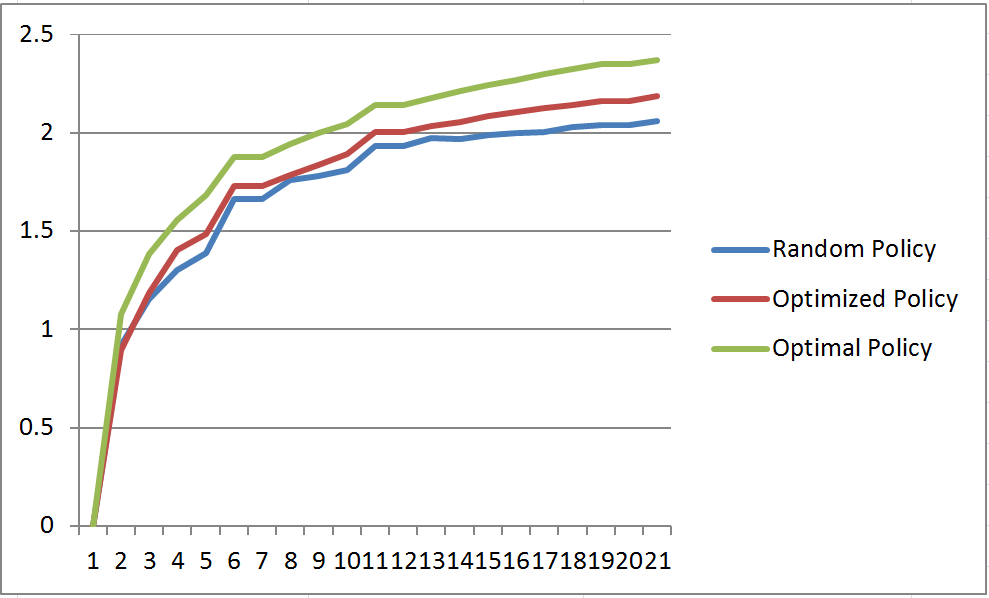
\includegraphics[width=\columnwidth]{img/q-values.png}
 \caption{Q-values for each episode, the X-axis shows the number of episodes and the Y-axis shows the log-scale Q-values.}
 \label{q-values}
 \end{figure}

\subsubsection{Dialog Evaluation} 
In addition to {task metrics}, we looked at {\em Dialog Metrics} to measure the number of turns for successful completions, and the number of words per turn.  

The average length of a dialog is 31.9 turns, the shortest completed dialog is 24 turns and the longest one is 43 turns. The length of the dialog is significantly larger than similar RL-based systems \cite{NjFunSingh02,young2010POMDP,frampton2009}. For Step 1, Step 2 abuse, Step 2 Dependence and Step 3, the average length of the dialog are respectively: 9.6, 4.8 and 13.4, and 4.1.
The average number of words used or recognized in each turn is 3.3. 
% HOW DOES THIS COMPARE TO OTHER WORKS?  
% this does NOT sound very good, only 3-4 words in each answer.

\subsection{Subjective Evaluation Results}

\subsubsection{User's experience}
After the subjects completed the intervention, the subjects answered a survey aimed at evaluating the user's experience with the system. The survey has two parts, the first part has 4 yes/no questions and the second part is a 34-item questionnaire about the subject's assessment and experience with the system. 

In the first part, we asked questions about reuse ``Would you use the system in future?", and ease of use ``Is the system easy to use and is it easy to understand how to use the system?", and ``Did the system understood what you said" and ``Did you know what to say to the system in each turn". Since these 4 questions are not directly related with dialog strategies and we want to see the complete picture, we did not compare test and training systems. 

Our evaluation of the subjective aspects shown in Figure \ref{yesNoEva} demonstrates that acceptability of the system by users is very high in terms of {\em Ease of Use} (81 Yes versus 8 No) and {\em Intention to Reuse} (63 Yes versus 26 No)
% DISCUSS ACTUAL NUMBERS, ADD UNIT IN FIGURE FOR Y AXIS, SAME FOR OTHER FIG BY THE WAY)
% NOT CLEAR HOW INTENTION TO REUSE WAS EVALUATED THOUGH, WHAT QUESTION(S)?
the system. The {\em What to say to system} shows that sometimes users do not know how to answer the system questions. We believe that the reason can be that when the system is in user initiative mode (open questions), the subjects may not be sure to what extend they should provide details. 
% DISCUSS: WHY DO YOU THINK THAT IS?  THE QUESTIONS WERE PRETTY SIMPLE, WHY DIDN'T THEY KNOW HOW TO ANSWER?
The {\em System understood} criteria shows that most of the users think that the system understood what they said.  We postulate that this is achieved with our ample use of confirmation questions that the system utters when not sure.

\subsubsection{Subjective Assessment of Speech Interfaces}

In the second part of the subjective assessment, we used a 34-item questionnaire named {\em Subjective Assessment of System Speech Interfaces (SASSI)} \cite{SASSI}. It is a widely used evaluation questionnaire in the SDS community. The subjects answered a randomized list of SASSI questionnaire on a 7-point Likert scale. The SASSI questionnaire queries 6 aspects of the user's assessment and experience with the system.  These aspects are \textit{Accuracy}, \textit{Likeability}, \textit{Cognitive Demand}, \textit{Annoyance}, \textit{Habitability}, and \textit{Speed} of the system. 


 \begin{figure}
 \centering
 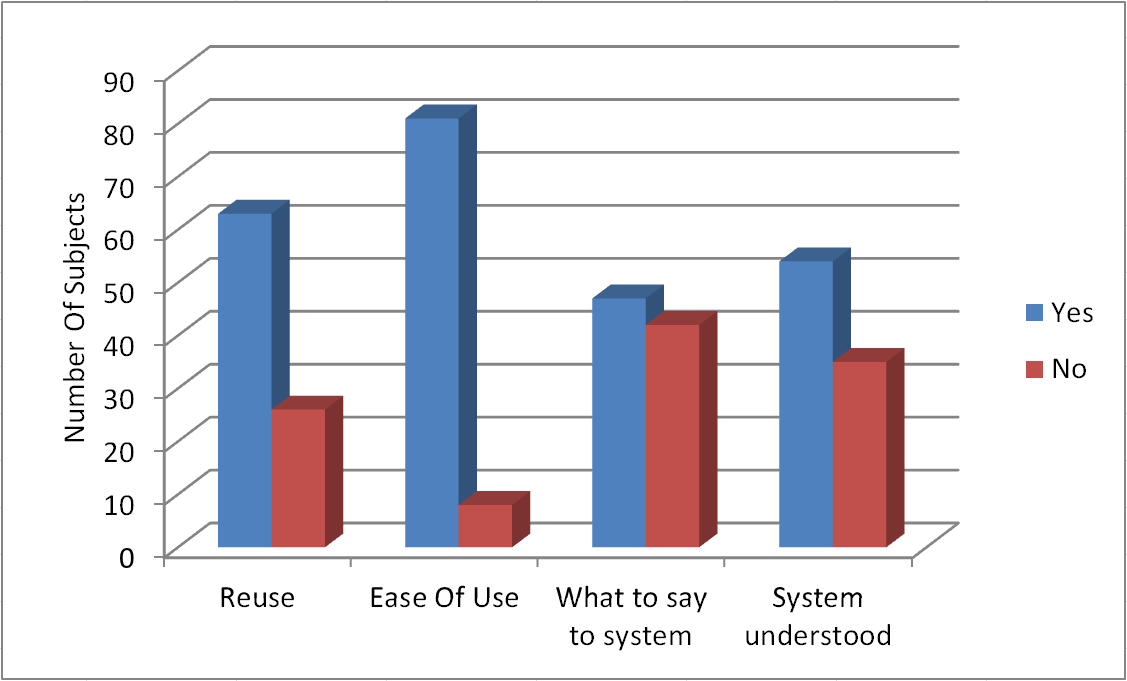
\includegraphics[width=\columnwidth]{img/subjective.png}
 \caption{Subjective Evaluation}
 \label{yesNoEva}
 \end{figure}
 

The items in \textit{Accuracy} are related to whether the system recognizes user's input correctly and does what the user expects. 
The items in {\em Likeability} include statements about the opinion and feelings of the user about the system. \textit{Cognitive Demand} summarizes the level of effort needed to use the system and the user's feelings arising from this effort. The \textit{Annoyance} includes statements such as ``the interaction with the system is repetitive/boring/irritating". \textit{Habitability} contains statements related to whether the user knows what to say and knows what the system is doing. The \textit{Speed} contains only 2 items related to the speed of the system. 
% RELATE TO PREVIOUS DISCUSSION ON USERS NOT KNOWING WHAT TO SAY.
We compared two versions of the system (training and testing) for the SASSI evaluation. As discussed earlier, \textbf{52} subjects used the training system and \textbf{37} subjects used the testing version of the system.

We show the results in Figure \ref{SASSI}. In the 7-point Likert scale, 1 is the lowest negative score (strongly disagree), 4 is neutral score (neither agree nor disagree) and 7 is the highest score (strongly agree).  
% I DON'T UNDERSTAND THE MEANING OF THE PARAGRAPH BELOW, TRY TO REPHRASE
We actually compared two versions of the system but our goal was also to assess the overall performance of the system for speed and habitability categories, because both versions of the system do not have any difference in terms of features which are assessed by speed and habitability measures. To be consistent, we compared habitability and speed measures, as we did for other subjective measures. The results for habitability and speed correlate our viewpoint, because the mean values are very close, as showed in Figure \ref{SASSI}.


\begin{figure}
\centering
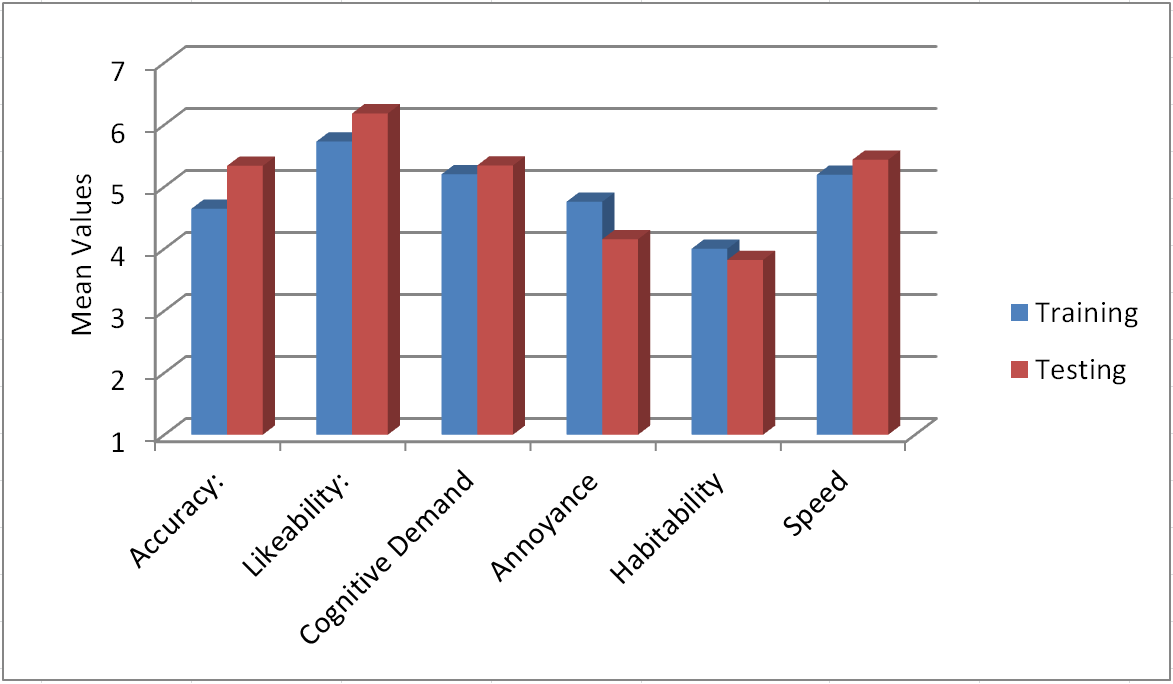
\includegraphics[width=\columnwidth]{img/SASSI.png}
\caption{Assessment - Negative (1) Neutral (4) Positive (7)}
\label{SASSI}
\end{figure}


In Table \ref{SASSIPVal}, we show mean values for each evaluation category for both versions of the system, the difference between mean values, and p-values. We obtained p-values by performing the standard two-sample t-test. Column 1 is the type of evaluation; Column 2 is the mean of the evaluated subjective category for training; Column 3 is the mean of the evaluated subjective category training (optimized) system; Column 4 shows the difference between test and training averages; and Column 5 is the statistical significance value obtained using the standard t-test.

{\em Accuracy} of the system improved in the test version: the results show that there is a statistical significance between the two versions ($p=0.0360 < 0.05$). This result indicates that the optimized system can select better dialog strategies then the training system which randomly selects dialog strategies.

\textit{Likeability} of the system improved slightly in the test version. As can be seen, both versions of the system have very high scores for likeability. It is possible to draw two conclusions: first the acceptance rate of the system is high; second, although the difference between the two versions is not statistically significant ($p=0.0928>0.05$), the optimized behavior of the system provides more desirable interactions.
 
The mean values of \textit{cognitive demand} and \textit{habitability} are very close for the training and testing versions (see Table \ref{SASSIPVal}). Therefore p-values are not statistically significant. However, we can infer that the required cognitive demand is slightly higher than neutral level for both versions. 
% WHAT IS THE 'NEUTRAL LEVEL'?
Habitability of the system is almost neutral for both of the versions.

We believe that there is a connection between \textit{accuracy} and \textit{annoyance} categories, because if the number of re-asks and confirmation increases, the annoyance level might increase. For the test version, the reported annoyance level decreased and the result is statistically significant ($p=0.0472<0.05$). Since the accuracy also increased for the test version, it might have had a significant impact on the decrease of annoyance. 
 
\begin{table}
\tabcolsep1.5mm
 %   \begin{tabular}{ | l | 1 | 1 | 1 | 1 |}
 \caption{Subjective Evaluation Categories: Training versus Testing} \label{SASSIPVal}
 \begin{tabular}{ | c | c | c | c | c | }
    \hline
    Evaluation Measure & Training & Testing & $\triangle$ & p-value \\ \hline
    Accuracy & 4.6435 & 5.3363 & 0.6928 & 0.0360  \\ \hline
    Likebility & 5.7286 & 6.1830 & 0.4544 & 0.0928 \\ \hline
    Cognitive Demand & 5.2000 & 5.3435 & 0.1435 & 0.6394 \\ \hline
    Annoyance & 4.7596 & 4.1540 & 0.6056 & 0.0472 \\ \hline
    Habitability & 4.000 & 3.8200 & 0.1800 & 0.6302 \\ \hline
    \end{tabular}
%    \begin{tabnote}
%    \Note{Column 1 is the type of evaluation; Column 2 is the mean of the evaluated subjective category for training; Column 3 is the mean of the evaluated subjective category training (optimized) system; Column 4 shows the difference between test and training averages; Column 5 is the statistical significance value obtained using the standard t-test}
%    \end{tabnote}
    \end{table} 


\section{Implications}

Health screening and assessment dialogs are different than dialogs that are found in information-seeking applications usually studied by SDS researchers. The main goal of brief behavior change interview dialogs is to collect initial screening information, educate patients, increase their awareness about potential problem behaviors and, if needed, refer the patient to a treatment. This is usually the plan of standardized health interviews (e.g.  \cite{humeniuk2010assist,steinberg2005brief,national2007helping}) by national or international health institutions. So the system has to conduct the conversation according to that plan. The system usually needs to ask one question at a time and in a specific order, while the flow of the dialog adapts according to the received answers. The length of the dialog is also longer than current information-seeking dialogs. 
 
Our work have several implications.  Our reduced state space representation with multiple MDPs enables to learn approximately optimal dialog policies with a relatively low amount of data. Even though we designed the system for brief alcohol interventions, the approach that we use is easily applicable to any other similar health interviews (e.g. eating behaviors, exercising behaviors, use of drugs). Indeed, brief interventions are adaptable and useful for a variety of life-style related issues that target one specific problematic behavior. 

Secondly, our collected dialog corpus will help the development of future data-driven research projects in the health domain.  

Thirdly, we connect this work with the notion of intelligent virtual agents (IVA).  Whereas we focussed our current discussion on our efficient approach for a spoken dialog-based interaction, our work is directly linked with our research on the graphical animation of the intelligent virtual agents that deliver the spoken intervention.  In a recent study  \cite{lisetti2013}, we showed that empathic virtual agents that deliver computer-based behavior change interventions are much more engaging than the currently available text-only computer-based interventions.  We created a model of empathic communication for an IVA to deliver behavior change interventions: in brief, the agent can sense the user's facial expressions and answers, and adjusts its non-verbal responses accordingly (e.g. express concern or encouragement) to deliver its messages.  Whereas there are debates about the impact of virtual characters communicating empathically with humans, our results showed that people are 31\% more likely to use our empathic agent system compared to using the same intervention content delivered instead with text-only.  We are currently in the process of integrating and evaluating our empathy agent model with the dialog manager discussed in this article.

Lastly, the performance of our system has also convinced medical and healthcare personnel to conduct randomized clinical trials to evaluate health outcomes and potentially deploy our system in clinicians' waiting rooms and community centers.  Whereas computer scientists might think that the healthcare profession could be threatened by the creation of such virtual counselor technologies, they are instead quite enthusiastic about getting technological assistance to address some of the nations' current epidemics (e.g. obesity, overweight, which put people at risk of a variety of chronic conditions such as diabetes, cardiovascular diseases, among others).  Virtual counselors have many advantages, including  increased accessibility to cost effective health interventions for people in need, increased anonymity and therefore self-disclosure of at-risk behaviors, which in turn leads to better healthcare, among many others \cite{lisetti2013}.

\section{Conclusion and Future Research}

We created a spoken embodied conversational system which uses the Reinforcement Learning (RL) paradigm for dialog management. The system is able to learn dialog strategies for initiative and confirmation selection. Our contributions to the SDS domain include the creation of a RL paradigm to the completely new domain of behavior change - where our dialog length is 4-5 times longer and where the nature of the dialog is less restricted than spoken dialog systems operated in tourist information domain.

We contributed to the healthcare domain with the first system to use speech as an input medium with a RL-based approach. Our initial evaluation showed that the dialog managers that are optimized with RL have the potential to reach optimal behavior, given enough training data. 
 
Our future research will involve extending our evaluation with more training data, and testing the optimized system with a larger number of subjects. Our system currently takes into account the best recognition of the speech recognizer.  We plan to use partial observability concepts to deal with uncertainty, which stems from speech recognizer hypotheses: future versions may work with N-best speech recognitions instead of best speech recognition. 


%\begin{acknowledgements}
%If you'd like to thank anyone, place your comments here
%and remove the percent signs.
%\end{acknowledgements}

% BibTeX users please use one of
%\bibliographystyle{spbasic}      % basic style, author-year citations
%\bibliographystyle{spmpsci}      % mathematics and physical sciences
\bibliographystyle{plain}       % APS-like style for physics
\bibliography{library}   % name your BibTeX data base


\end{sloppy}
\end{document}
% end of file template.tex

